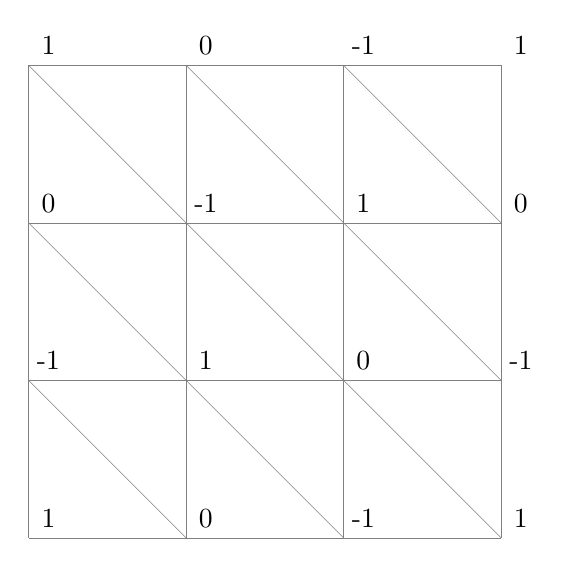
\begin{tikzpicture}
	\foreach \i [evaluate={\ii=int(\i-1);}] in {0,...,3}{
			\foreach \j [evaluate={\jj=int(\j-1);}] in {0,...,3}{
					\coordinate [shift={(2*\j,2*\i)}] (n-\i-\j) at (0:0);

					\ifnum\i>0
						\draw [help lines] (n-\i-\j) -- (n-\ii-\j);
					\fi
					\ifnum\j>0
						\draw [help lines] (n-\i-\j) -- (n-\i-\jj);
						\ifnum\i>0
							\draw [help lines] (n-\ii-\j) -- (n-\i-\jj);
						\fi
					\fi

					% Add labels on diagonals
					\ifnum\i=\j
						\node at ([shift={(0.25,0.25)}]n-\i-\j) {1};
					\fi
					\ifnum\i=\numexpr\j-1\relax
						\node at ([shift={(0.25,0.25)}]n-\i-\j) {0};
					\fi
					\ifnum\i=\numexpr\j-2\relax
						\node at ([shift={(0.25,0.25)}]n-\i-\j) {-1};
					\fi
					\ifnum\i=\numexpr\j-3\relax
						\node at ([shift={(0.25,0.25)}]n-\i-\j) {1};
					\fi
					\ifnum\i=\numexpr\j+1\relax
						\node at ([shift={(0.25,0.25)}]n-\i-\j) {-1};
					\fi
					\ifnum\i=\numexpr\j+2\relax
						\node at ([shift={(0.25,0.25)}]n-\i-\j) {0};
					\fi
					\ifnum\i=\numexpr\j+3\relax
						\node at ([shift={(0.25,0.25)}]n-\i-\j) {1};
					\fi
				}}
\end{tikzpicture}